
\documentclass{article}
\usepackage{epsfig,graphics,fancybox,amsmath,hyperref,ulem,tabularx,color,graphicx}

\setlength{\textwidth}{6.5in}
\setlength{\textheight}{8.5in}
\setlength{\parindent}{0pt}

\begin{document}
\setlength{\topmargin}{0pt}
\setlength{\oddsidemargin}{0pt}

Recall that the overall hypotheses we want to test are
$$H_0: \beta_1=\beta_2=0 ~~vs~~H_A: \text{ at least one is non-zero}$$
This is the test done in the ANOVA table given in the output from a MLR model.  This is called the \textbf{global $F$-test} as it tests whether at least one of the terms in the model is important for predicting the response.\\~\\

The ANOVA table for MLR follows the same ideas as in SLR.  We are taking the total amount of variation in the response (SS(Tot)) and partitioning it into a part due to the model (SS(R)) and a part due to experimental error (SS(E)).  In fact, the formulas for the sums of squares remain the same, only the degrees of freedom and the $F$-distribution used for finding the p-value change.\\~\\

The full ANOVA table for MLR is given below:\\
\begin{tabular}{|c|c|c|c|c|} \hline
Source & Sum of squares & df & Mean Square & F-Ratio \\ \hline
Regression & $SS(R)$ & p & $MS(R)$ & $MS(R)/MS(E)$ \\
Error & $SS(E)$ & $n-p-1$ & $MS(E)$ &  \\
Total & $SS(Tot)$ & $n-1$ & &  \\ \hline
\end{tabular}
~\\
\textbf{How to do MLR in SAS?}\\
The following code will produce output appropriate for analysis:
\begin{small}
\begin{verbatim}
proc reg data=adexp ;
model adsorp=aluminum iron/clb;
run;
\end{verbatim}
\end{small}

\begin{center}
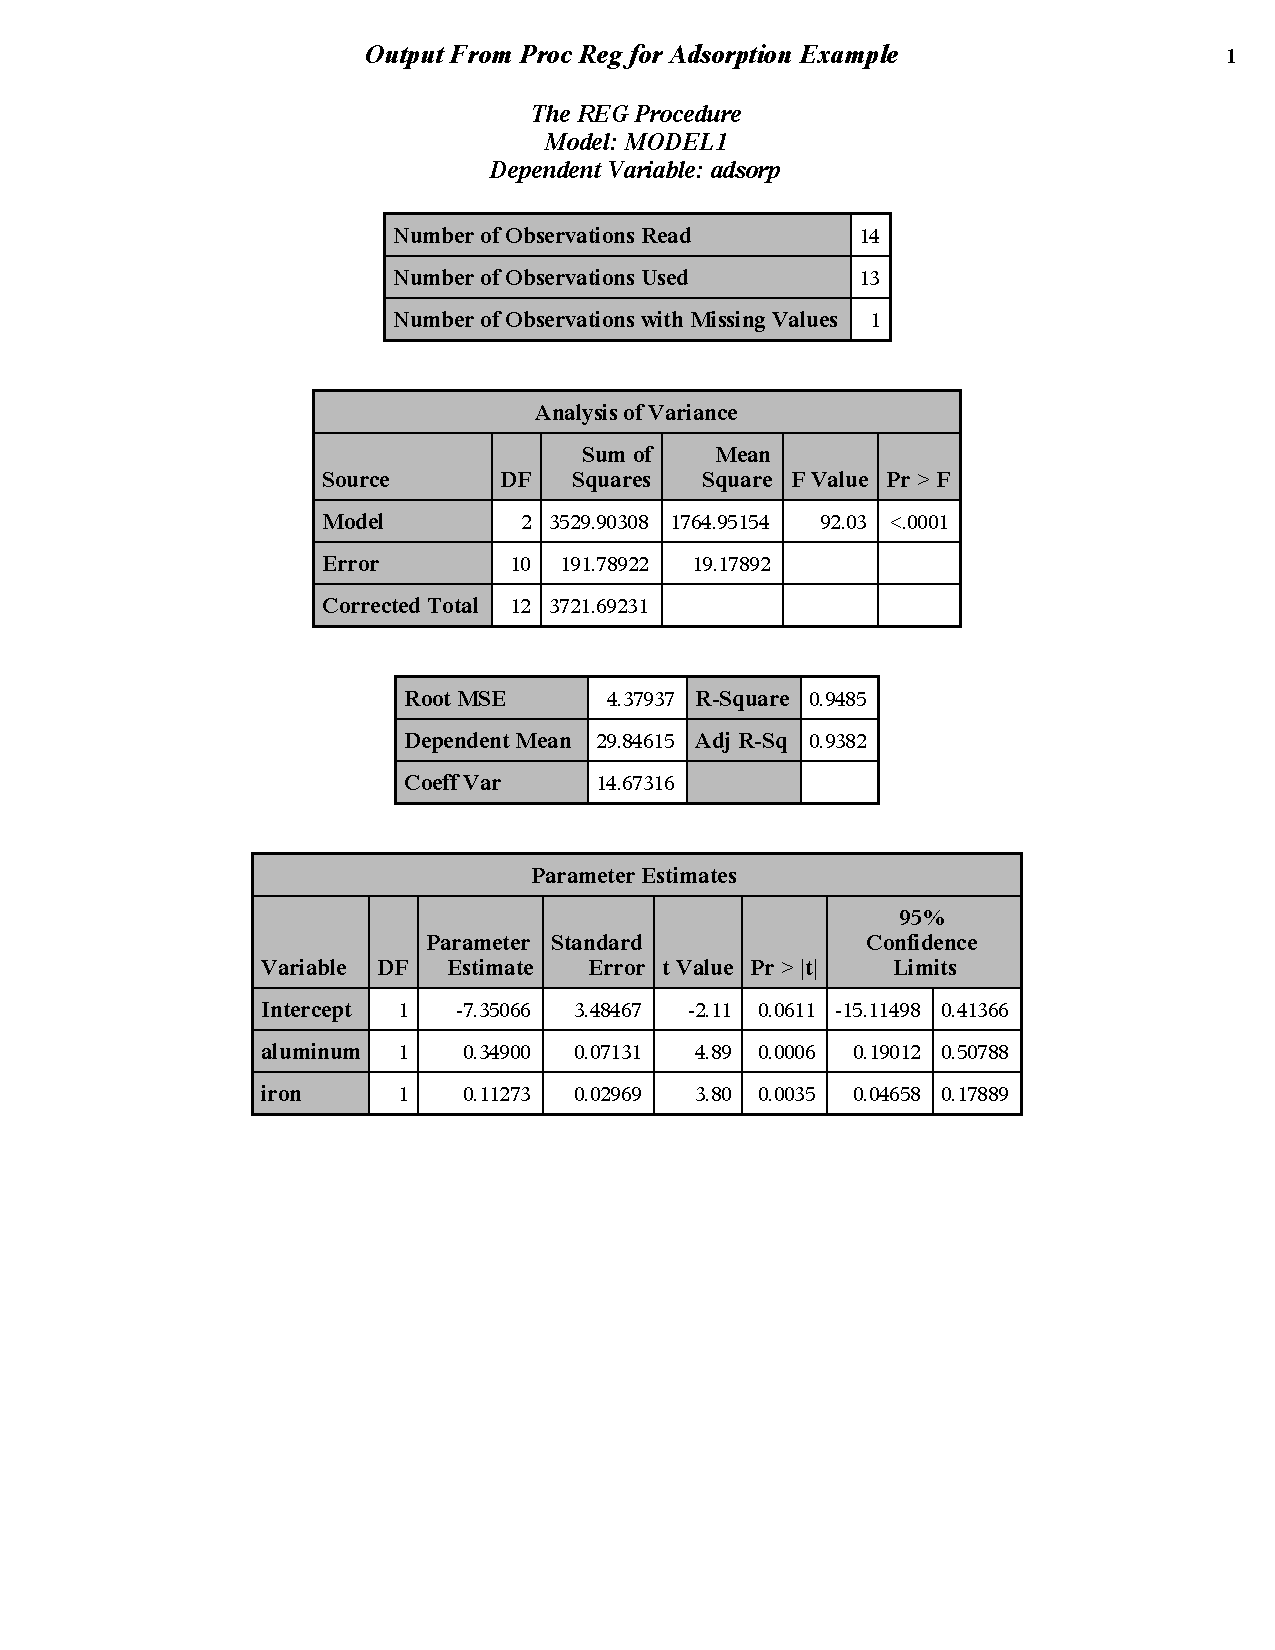
\includegraphics[page=1,scale=0.55,trim = 20mm 70mm 20mm 0mm]{mlradexp}\\
\end{center}

\textit{\textcolor{red}{Note!  The tests in the parameter estimate table are tests for that $\beta$ coefficient being 0 \textbf{after accounting for the other predictors in the model}.}}

\begin{center}
\includegraphics[page=2,scale=0.55,trim = 20mm 60mm 20mm 0mm]{mlradexp}\\
\includegraphics[page=3,scale=0.4,trim = 20mm 120mm 20mm 20mm]{mlradexp}
\end{center}

\newpage

\textbf{A non-additive model example:}\\
A random sample of students taking the same exam:
\begin{center}
\begin{tabular}{|c|c|c|} \hline
IQ & Study TIME & GRADE \\ \hline
105 & 10 & 75 \\
110 & 12 & 79 \\
120 & 6 & 68 \\
116 & 13 & 85 \\
122 & 16 & 91 \\
130 & 8 & 79 \\
114 & 20 & 98 \\
102 & 15 & 76 \\ \hline
\end{tabular}
\end{center}

Consider regressing GRADE on IQ ($X_1$), TIME($X_2$), and TI ($X_1*X_2$), where TI = TIME*IQ.  That is, we fit the model:
$$Y=\beta_0+\beta_1X_1 +\beta_2X_2+\beta_3X_1X_2+E$$
\begin{small}
\begin{verbatim}
proc reg;
model Grade = IQ Time TI;
run;

                                      The SAS System                                     1
                                    The REG Procedure

                                   Analysis of Variance
 
                                          Sum of           Mean
      Source                   DF        Squares         Square    F Value    Pr > F

      Model                     3      610.81033      203.60344      26.22    0.0043
      Error                     4       31.06467        7.76617                   
      Corrected Total           7      641.87500                                    

                                   Parameter Estimates
 
                    Parameter     Standard
   Variable   DF     Estimate        Error  t Value  Pr > |t|
   Intercept   1     72.20608     54.07278     1.34    0.2527
   IQ          1     -0.13117      0.45530    -0.29    0.7876
   Time        1     -4.11107      4.52430    -0.91    0.4149
   TI          1      0.05307      0.03858     1.38    0.2410 
\end{verbatim}
\end{small}

Discussion of the interaction model:\\
 We call the product TI = Time*IQ an "interaction" term. That is, our explanatory variables do not have an independent effect on the response.
$$ \widehat{Mean Grade} = 72.21 - 0.13*IQ - 4.11*Time + 0.0531*TI$$ 
Now if IQ = 100 we get
$$ \widehat{Mean Grade} = (72.21 - 13.1) + (- 4.11 + 5.31)*Time$$
and if IQ  120 we get
$$ \widehat{Mean Grade} = (72.21 - 15.7) + (- 4.11 + 6.37)*Time.$$
Thus we expect an extra hour of study to increase the grade by 1.20 points for someone with IQ = 100 and by 2.26 points for someone with IQ = 120 if we use this interaction model.\\~\\
Generally, we can interpret the (true) $\beta$ parameters in the model as:
\begin{itemize}
\item $\beta_0$ - Average value of Grade when IQ and Study Time are 0
\item $\beta_1$ - Average change in Grade for a unit increase in IQ when Study Time is 0
\item $\beta_2$ - Average change in Grade for a unit increase in Study Time when IQ is 0
\item $\beta_3$ - Average change in the slope for IQ (or Study Time) for a given value of Study Time (or IQ).
\end{itemize}
The interpretation of the interaction `slope' can be seen by looking at the following:
$$\mu(x_1+1,x_2)-\mu(x_1,x_2)=\beta_0+\beta_1(x_1+1)+\beta_2x_2+\beta_3(x_1+1)(x_2)-\beta_0-\beta_1x_1-\beta_2x_2-\beta_3x_1(x_2)$$
$$=\beta_1+\beta_3x_2$$
So $\beta_3$ is the amount the slope for $x_1$ changes per unit change in $x_1$ while $x_2$ is held constant.\\~\\

Note:  The global p-value is significant, but none of our individual terms are.   This gives evidence that our model is over-fit.  we may want to go back to the simpler ``main effects'' model.  \\~\\

\textit{\textcolor{red}{The next idea to tackle is what model to use if we are unsure of the predictors we want in our model.  This idea is called \textbf{model selection}.}}\\~\\

\newpage

\textbf{Model Selection:}\\

$x_1,x_2,x_3$ denote $p$ independent variables.  Consider
several models:
\begin{enumerate}
\item $\mu(x_1,x_2,x_3) = E(Y|x_1,x_2,x_3) =  \beta_0 + \beta_1 x_1$
\item $\mu(x_1,x_2,x_3) = E(Y|x_1,x_2,x_3) =  \beta_0 + \beta_2 x_2$
\item $\mu(x_1,x_2,x_3) = E(Y|x_1,x_2,x_3) =  \beta_0 + \beta_3 x_3$
\item $\mu(x_1,x_2,x_3) = E(Y|x_1,x_2,x_3) =  \beta_0 + \beta_1 x_1 + \beta_2 x_2 + \beta_3 x_3$
\item $\mu(x_1,x_2,x_3) = E(Y|x_1,x_2,x_3) =  \beta_0 + \beta_1 x_1 + \beta_3 x_3$
\item $\mu(x_1,x_2,x_3) = E(Y|x_1,x_2,x_3) =  \beta_0 + \beta_1 x_1 + \beta_2 x_2$
\item $\mu(x_1,x_2,x_3) = E(Y|x_1,x_2,x_3) =  \beta_0 + \beta_2 x_2 + \beta_3 x_3$
\end{enumerate}
$A$ is nested in $B$ means model $A$ can be obtained by restricting (e.g. setting to 0 \textcolor{red}{or setting equal $\beta$'s}) parameter values in model $B$.

\textbf{True or false:}
\begin{itemize}
\item Model 1 nested in Model 4 \textcolor{red}{True}~~~~~~~Model 1 nested in Model 5 \textcolor{red}{True}
\item Model 2 nested in Model 4 \textcolor{red}{True}~~~~~~~Model 4 nested in Model 1 \textcolor{red}{False}
\item Model 3 nested in Model 4 \textcolor{red}{True}~~~~~~~Model 5 nested in Model 4 \textcolor{red}{True}
\item Model 3 nested in Model 7 \textcolor{red}{True}~~~~~~~Model 1 nested in Model 7 \textcolor{red}{False}
\end{itemize}

$A$ nested in $B$ $\longrightarrow$ $A$ called {\em reduced model}, $B$ called {\em full model}.  \\~\\

$p$ - number of regression parameters in full model  \\
$q$ - number of regression parameters in reduced model \\
$p-q$ - number of regression parameters being tested. \\~\\

\textcolor{red}{In comparing two models, suppose
\begin{center}
$\beta_1,\ldots,\beta_q$ in reduced model ($A$)\\
$\beta_1,\ldots,\beta_q,\beta_{q+1},\ldots,\beta_p$ in full model ($B$).
\end{center}
~\\Comparison of models $A$ and $B$ amounts to testing
$$H_0: \beta_{q+1} = \beta_{q+2} = \ldots = \beta_{p} =0 \text{ (model $A$ ok)}$$
$$H_1: \beta_{q+1} , \beta_{q+2} , \ldots , \beta_{p} \text{ not all 0 (model $B$ adds something)}$$
To test this hypothesis we can use the $F$ distribution with $p-q$ numerator df and $n-p-1$ denominator df
$$F = \frac{(SS(E)_r - SS(E)_f)/(p-q)}{MS(E)_f}=\frac{(SS(R)_f - SS(R)_r)/(p-q)}{MS(E)_f}$$
($r$ and $f$ abbreviate {\em reduced} and {\em full}, respectively.)\\~\\
Difference in the numerator called an \textbf{extra regression sum of squares}:
$$ R(\beta_{q+1},\beta_{q+2},\ldots,\beta_p|\beta_0,\beta_{1},\beta_{2},\ldots,\beta_q) = SS(R)_f-SS(R)_r.$$
(ok to supress $\beta_0$ in these extra $SS$ terms.)}\\

\textit{\textcolor{blue}{Consider why this test stat makes sense.  $SS(R)_f-SS(R)_r$ can be thought of as the amount of variation in $Y$ (or part of SS(Tot)) that can be attributed to the variables in the alternative hypothesis.  If the variables in the alternative are really meaningful, this should a relatively large quantity compared to MS(E).}}\\

Let`s get a handle on this notation.  Give the extra regression $SS$ terms for comparing some of the nested models on preceding page:
\begin{itemize}
\item Model 1 in model 4: $R(\beta_2,\beta_3|\beta_1)$
\item Model 2 in model 4: \textcolor{red}{$R(\beta_1,\beta_3|\beta_2) $} 
\item Model 3 in model 4: \textcolor{red}{$R(\beta_1,\beta_2|\beta_3) $} 
\item Model 1 in model 5: $R(\beta_3|\beta_1) $
\item Model 5 in model 4: \textcolor{red}{$R(\beta_2|\beta_1,\beta_3) $}
\end{itemize}

\textbf{An example: How to measure body fat?} For each of $n=20$ healthy individuals, the following measurements were made: bodyfat percentage $y_i$, triceps skinfold thickness, $x_{1}$, thigh circumference $x_{2}$, midarm circumference $x_{3}$.
\begin{small}
\begin{verbatim}
  x1    x2    x3    y
  19.5  43.1  29.1  11.9
  24.7  49.8  28.2  22.8                   ods graphics on;
  30.7  51.9  37.0  18.7                   proc corr plots=matrix;
  29.8  54.3  31.1  20.1                   var y x1 x2 x3;
  19.1  42.2  30.9  12.9                   run;
  25.6  53.9  23.7  21.7
  31.4  58.5  27.6  27.1
  27.9  52.1  30.6  25.4
  22.1  49.9  23.2  21.3
  25.5  53.5  24.8  19.3
  31.1  56.6  30.0  25.4
  30.4  56.7  28.3  27.2
  18.7  46.5  23.0  11.7
  19.7  44.2  28.6  17.8
  14.6  42.7  21.3  12.8
  29.5  54.4  30.1  23.9
  27.7  55.3  25.7  22.6
  30.2  58.6  24.6  25.4
  22.7  48.2  27.1  14.8
  25.2  51.0  27.5  21.1
\end{verbatim}
\end{small}

\begin{center}
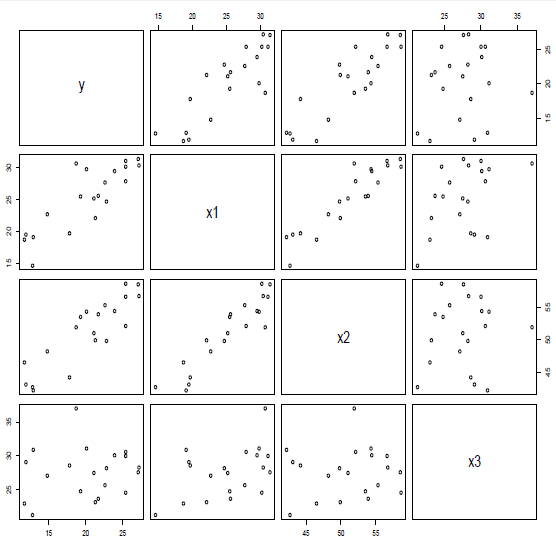
\includegraphics[height=3.7in,width=3.7in]{bodyfat}
\end{center}
\begin{small}
\begin{verbatim}
                Pearson Correlation Coefficients, N = 20 
                        Prob > |r| under H0: Rho=0
 
                       y            x1            x2            x3

        y        1.00000       0.84327       0.87809       0.14244
                                <.0001        <.0001        0.5491

        x1       0.84327       1.00000       0.92384       0.45778
                  <.0001                      <.0001        0.0424

        x2       0.87809       0.92384       1.00000       0.08467
                  <.0001        <.0001                      0.7227

        x3       0.14244       0.45778       0.08467       1.00000
                  0.5491        0.0424        0.7227              
\end{verbatim}
\end{small}

Looking at the scatter plots and the correlation output, marginal associations between $y$ and $x_1$ and between
$y$ and $x_2$ are highly significant, providing evidence of a strong $r\approx 0.85$ linear association between average
bodyfat and triceps skinfold and between average bodyfat and thigh circumference.\\~\\

Notice the scatter plot between $x_1$ and $x_2$, there is a strong linear relationship.  This means that triceps skinfold and thigh circumference are giving some of the same information.  This can lead to issues when fitting a model.\\~\\
\textbf{Multicollinearity:} linear associations among the independent variables; causes problems such as inflated sampling variances for $\hat{\boldsymbol{\beta}}$.

\begin{small}
\begin{verbatim}
proc reg data=bodyfat;
   model y=x1/covb;
   model y=x2/covb;
   model y=x3/covb;
   model y=x1 x2/covb;
   model y=x1 x2 x3/covb;
run;
\end{verbatim}
\end{small}
Yields the following output:
\begin{center}
\begin{tabular}{cc}
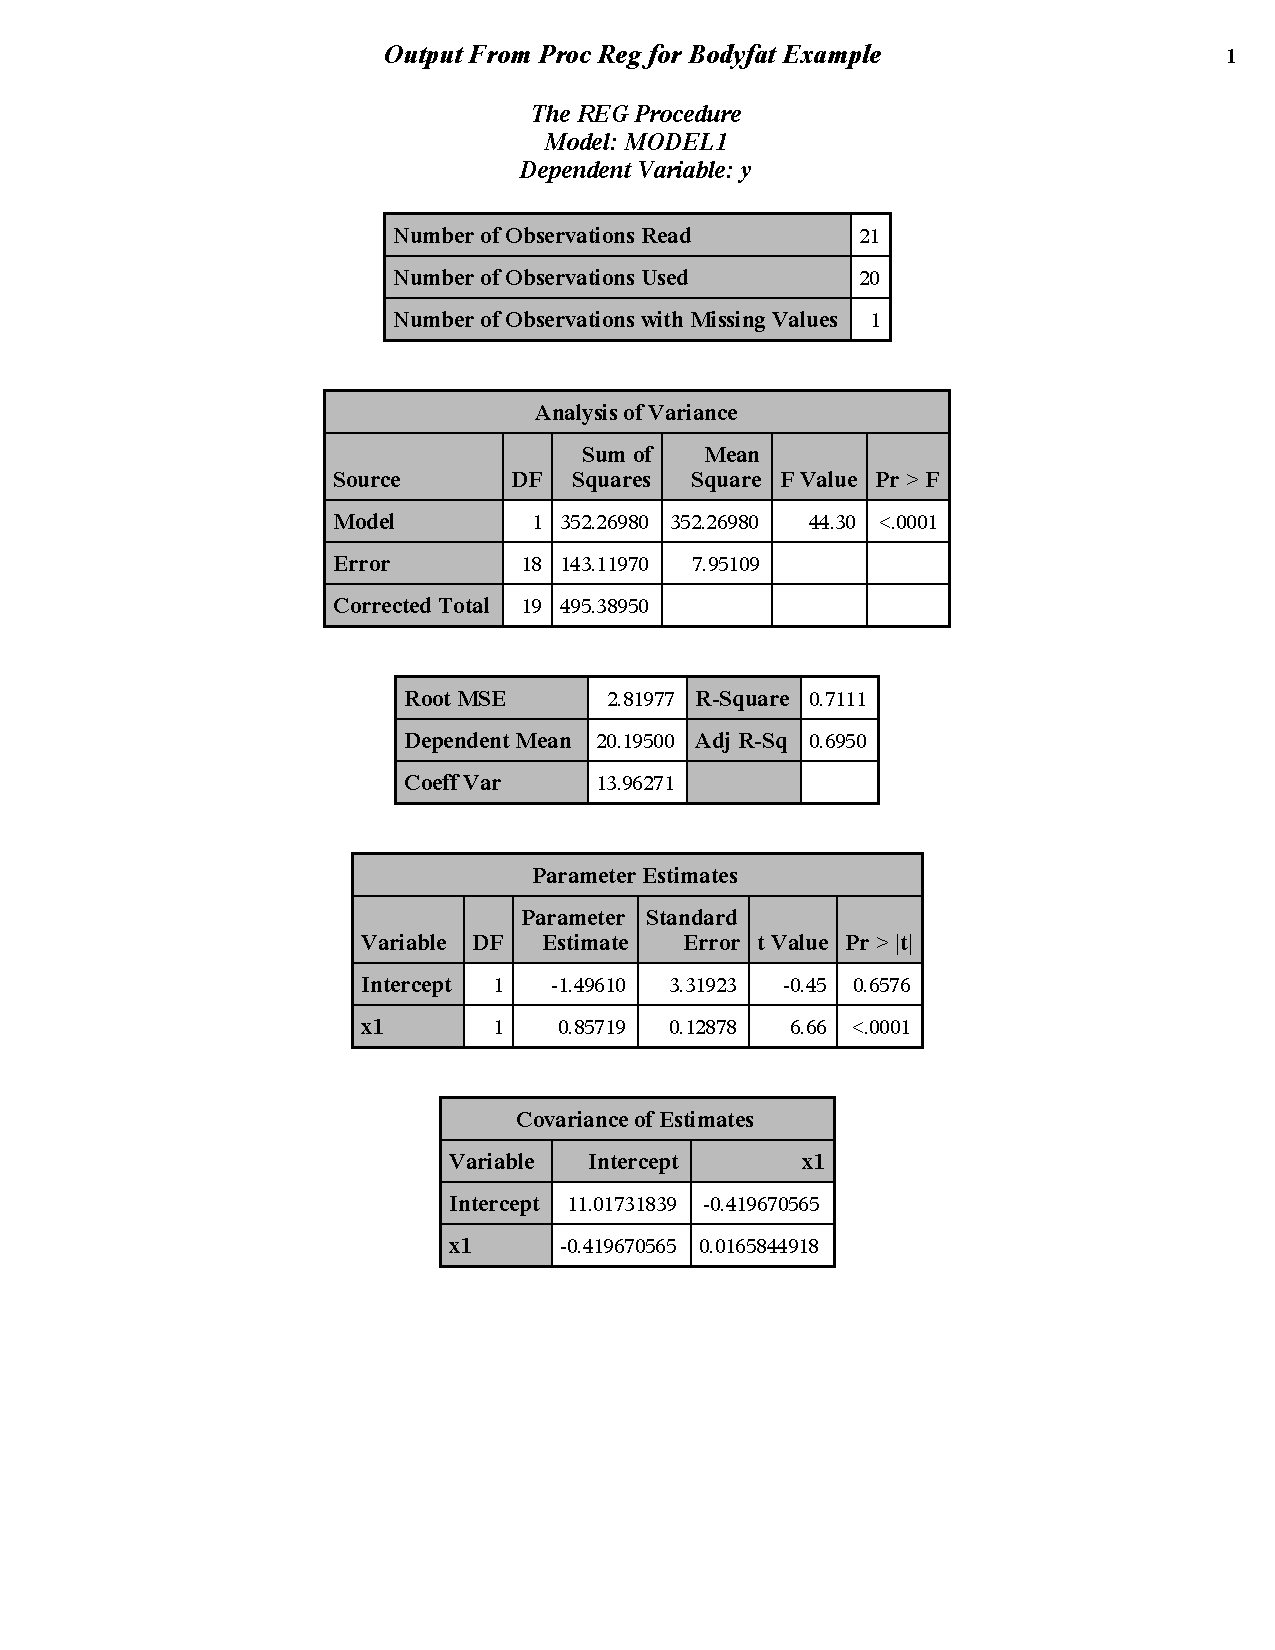
\includegraphics[page=1,scale=0.5,trim=40mm 30mm 20mm 10mm]{bodyfatexample}&
\includegraphics[page=2,scale=0.5,trim=40mm 30mm 20mm 10mm]{bodyfatexample}\\
\end{tabular}
\begin{tabular}{cc}
\includegraphics[page=3,scale=0.5,trim=40mm 30mm 20mm 10mm]{bodyfatexample}&
\includegraphics[page=4,scale=0.5,trim=40mm 30mm 20mm 10mm]{bodyfatexample}\\
\end{tabular}
\includegraphics[page=5,scale=0.6,trim=40mm 30mm 20mm 10mm]{bodyfatexample}
\end{center}

Question:  Why is the global p-value in the last model significant, i.e. at least one predictor is useful, but the individual tests are all nonsignificant?\\~\\

\textcolor{red}{Each individual test is a test for that variable given the other factors are retained in the model.}\\~\\

\textit{\textcolor{red}{Output and significance results discussed.  Note the covariance of the parameter estimates are inflated in the last model.  This is exactly the type of situation where we might want to employ a model selection strategy.}}\\~\\

In the bodyfat data, consider comparing the simple model that $Y$ depends only on $x_1$ (triceps) versus the full model that it depends on all three.
\begin{eqnarray*}
\mbox{Model } A: \mu(x_1,x_2,x_3) & = & \beta_0 + \beta_1 x_1 \\
\mbox{Model } B: \mu(x_1,x_2,x_3) & = & \beta_0 + \beta_1 x_1 + \beta_2 x_2 + \beta_3 x_3 
\end{eqnarray*} 
or the null hypothesis 
$$H_0: \beta_2=\beta_3=0 \ \ \mbox{  vs  } \ \ H_1: \beta_2, \beta_3 \mbox{ not both }0$$ 
after accounting for $x_1$.
Our $F$ statistic can be used
$$ F = \frac{(396.9-352.3)/2}{6.15} = \frac{22.3}{6.15}=3.64$$
How many $df$ for numerator and denominator? \\~\\
The $95^{th}$ percentile is $F(0.05,\textcolor{red}{2} ,\textcolor{red}{16}) = 3.63$.\\~\\
Our conclusion about the hypotheses?\\
\textcolor{red}{Reject $H_0$ in favor of $H_A$.  The full model gives us something more than just the SLR model with x1.}\\
That is, after accounting for the linear dependence between triceps and bodyfat, there is still some linear association between mean bodyfat and at least one of $x_2,x_3$ (thigh,midarm).  \\~\\

\textbf{To get the nested model $F$-ratio in SAS:}
\begin{small}
\begin{verbatim}
proc reg data=bodyfat;
     model y=x1 x2 x3;
     test x2=0,x3=0;
run;
\end{verbatim}
\end{small}

\begin{center}
\includegraphics[page=4,scale=0.6,trim= 10mm 200mm 10mm 10mm]{bodyfatexampletriceps}
\end{center}

However, we saw in the previous output that a model with all three variables is no good.  This is due to the multicollinearity.  We will now very briefly look at a few automated model selection techniques.\\~\\

\newpage
\textbf{Using proc reg to perform variable selection:}\\
We`ll discuss three hypothesis testing methods for selecting variables (there are many other ways to accomplish this we won`t discuss).
\begin{enumerate}
\item \textbf{Forward Selection} - Start with nothing and work forward.
	\begin{enumerate}
		\item Begin with a model with only $\beta_0$
		\item Calculate $R(\beta_i|\beta_0)$ for all possible predictors and find p-values for each
		\item Take most significant p-value less than a cutoff (say 0.3), add predictor into model.  
		\item Say $\beta_j$ was added in the last step, repeat above process with added predictor.  That is, calculate $R(\beta_i|\beta_0,\beta_j)$ for all other predictors, etc.
		\item Stop when no predictors are below the cutoff or if the full model is selected.
	\end{enumerate}
\item \textbf{Backward Selection} - Start with everything and work backward. 
\begin{enumerate}
		\item Start with full model.
		\item Locate variable with largest p-value greater than a cutoff (say 0.1), remove that variable.
		\item Repeat until all p-values are less than the cut off or the null model (intercept only model) is chosen.
	\end{enumerate}
\item \textbf{Subset Selection} - Compute all possible models, pick best.
\begin{enumerate}
		\item Compare each of the models using a criterion.
		\item Choose model that minimizes that criterion.  Possible criteria include:
		\begin{itemize}
			\item $Adjusted~R^2 = 1-\frac{n-1}{n-p-1}(1-R^2)$ (takes into account the addition of more predictors)
			\item Mallow`s $C_P$, AIC, AICc, or BIC (all take into account the model complexity, not just how well the model fits the data)
		\end{itemize}
	\end{enumerate}
\end{enumerate}

\textbf{How to do these model selection methods in SAS?}\\
\begin{small}
\begin{verbatim}
proc reg data=bodyfat plots=none;
    model y=x1 x2 x3/selection=cp ;
    model y=x1 x2 x3/selection=forward SLentry=0.3;
    model y=x1 x2 x3/selection=backward SLstay=0.1;
  	model y=x1 x2 x3/selection=adjrsq;
run;
\end{verbatim}
\end{small}

\begin{center}
\begin{tabular}{cc}
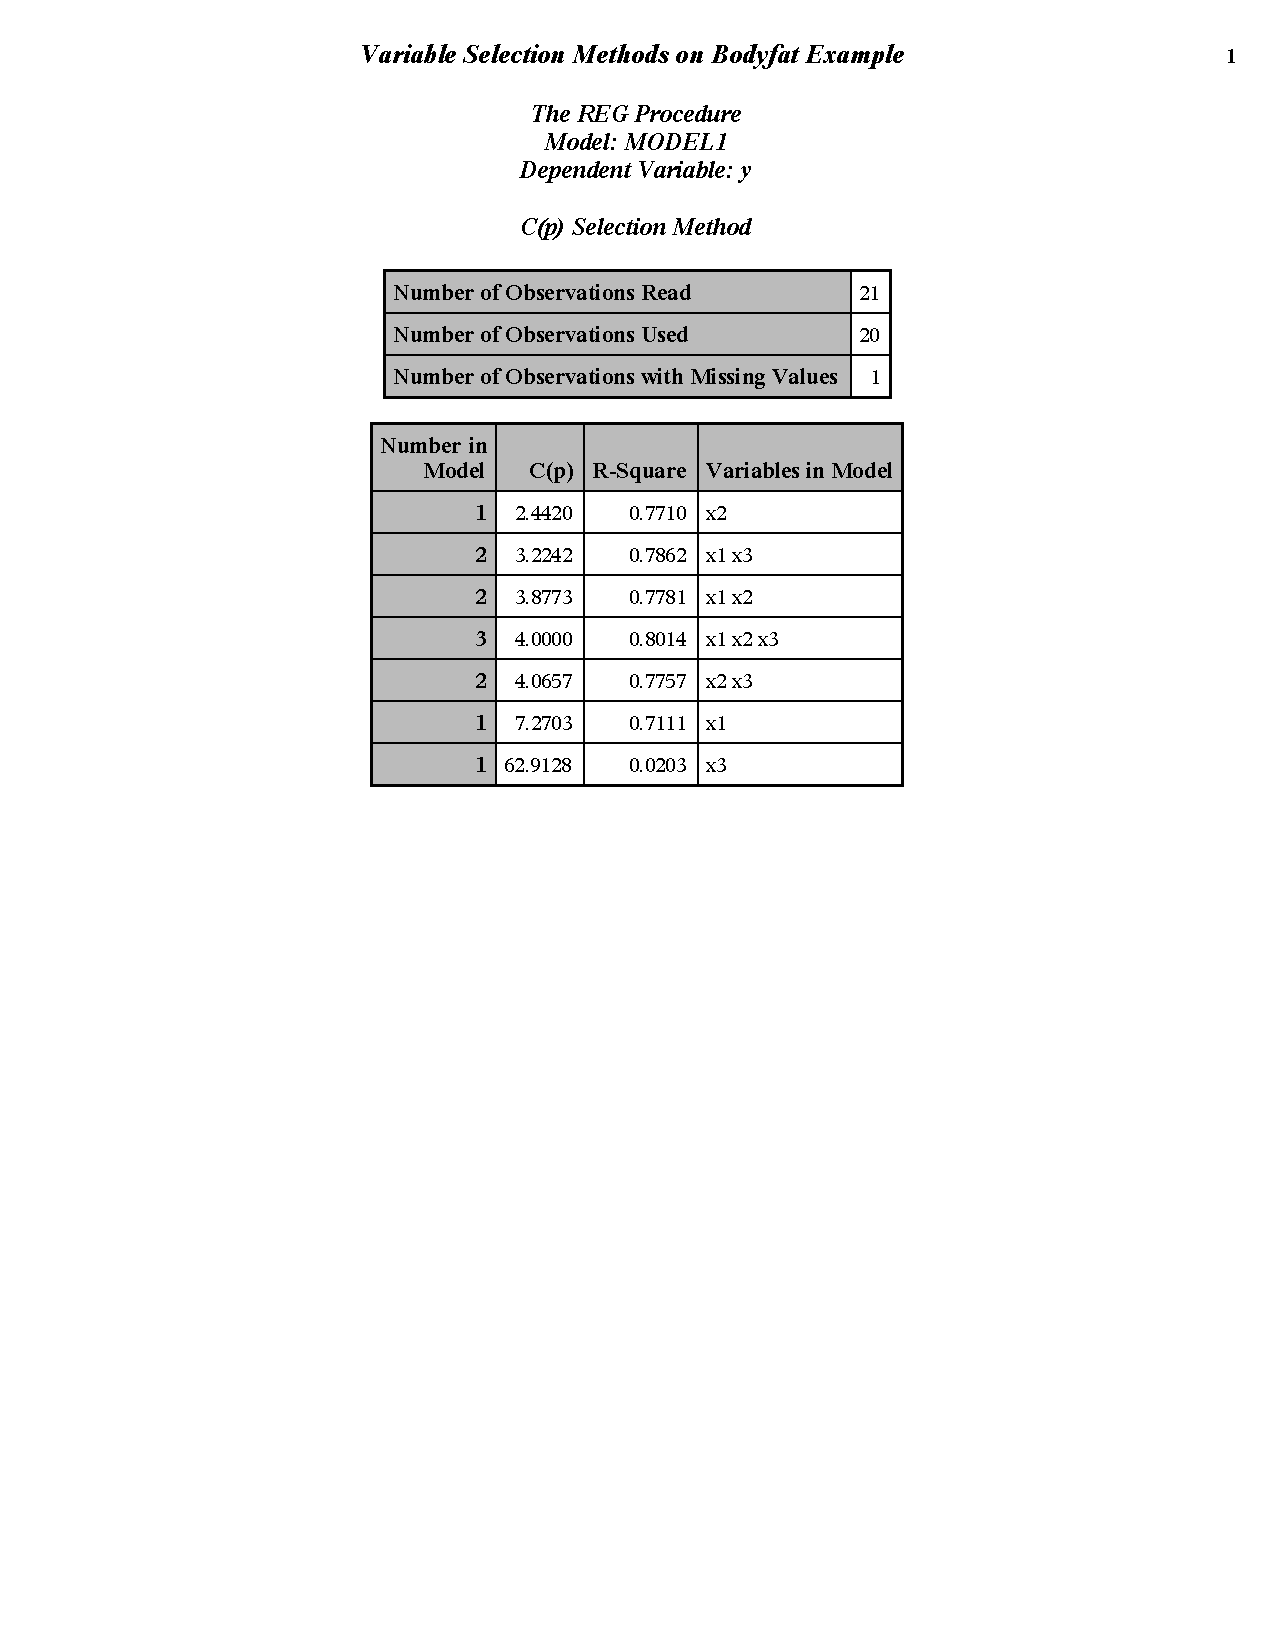
\includegraphics[page=1,scale=0.6,trim=40mm 30mm 20mm 10mm]{bodyfatexampleselection}&
\includegraphics[page=2,scale=0.6,trim=40mm 30mm 20mm 10mm]{bodyfatexampleselection}\\
\end{tabular}
\begin{tabular}{cc}
\includegraphics[page=3,scale=0.6,trim=40mm 30mm 20mm 10mm]{bodyfatexampleselection}&
\includegraphics[page=4,scale=0.6,trim=40mm 30mm 20mm 10mm]{bodyfatexampleselection}\\
\end{tabular}
\includegraphics[page=5,scale=0.6,trim=40mm 150mm 20mm 10mm]{bodyfatexampleselection}
\end{center}

\textit{\textcolor{red}{Models selected discussed.  Notice that they are not the same.  You should bring some subject matter knowledge into play here.\\~\\
If you notice, we now really have multiple tests for a given slope term.  A different test for each set of variables already being accounted for.  Let`s discuss this idea in more detail.}}\\~\\

\textbf{Types of Sums of Squares}\\
Given that we have 4 predictors, $X_1-X_4$ we really can have a number of tests based on nested models for $\beta_4=0$ (or for any other $\beta$ for that matter).  Let`s write them down in terms of extra regression sums of squares:\\
$R(\beta_4|\beta_0)$ (SLR test)\\
$R(\beta_4|\beta_0,\beta_1)$ (test after accounting for $X_1$)\\
$R(\beta_4|\beta_0,\beta_2)$ (test after accounting for $X_2$)\\
$R(\beta_4|\beta_0,\beta_3)$ (test after accounting for $X_3$)\\
$R(\beta_4|\beta_0,\beta_1,\beta_2)$ (test after accounting for $X_1$ and $X_2$)\\
$R(\beta_4|\beta_0,\beta_1,\beta_3)$ (test after accounting for $X_1$ and $X_3$)\\
$R(\beta_4|\beta_0,\beta_2,\beta_3)$ (test after accounting for $X_2$ and $X_3$)\\
$R(\beta_4|\beta_0,\beta_1,\beta_2,\beta_3)$ (test after accounting for $X_1$, $X_2$, and $X_3$)\\~\\
Some of these tests can be easily found using different types of sums of squares.\\~\\

\textcolor{red}{
\begin{itemize}
\item Type I sums of squares - sequential, test for adding the variable after all \textit{previous} variables are accounted for (order of variables in model determine the tests).
\item Type II sums of squares - partial, test for adding the variable once all other terms not containing a function of that variable are accounted for (i.e. interactions/quadratics/etc).
\item Type III sums of squares - partial, test for adding the variable after all other terms in the model are accounted for.
\end{itemize}
}

The tests given for the parameter estimates are all type III tests and this is the test usually done to determine if a slope term has significance.  However, type I tests are very useful for model building.  For example, if we wanted to look at building a model for the bodyfat example and we thought the order of importance for the variables was $X_1$ (triceps), $X_3$ (midarm), and $X_2$ (thigh), we could get sequential tests for these models using type I sums of squares.\\~\\ 

In SAS proc reg use the following code:\\
\begin{small}
\begin{verbatim}
proc reg data=bodyfat;
   model y=x1 x3 x2/ss1; *Note the order of variables is important for Type I;  
run;
\end{verbatim}
\end{small}

\begin{center}
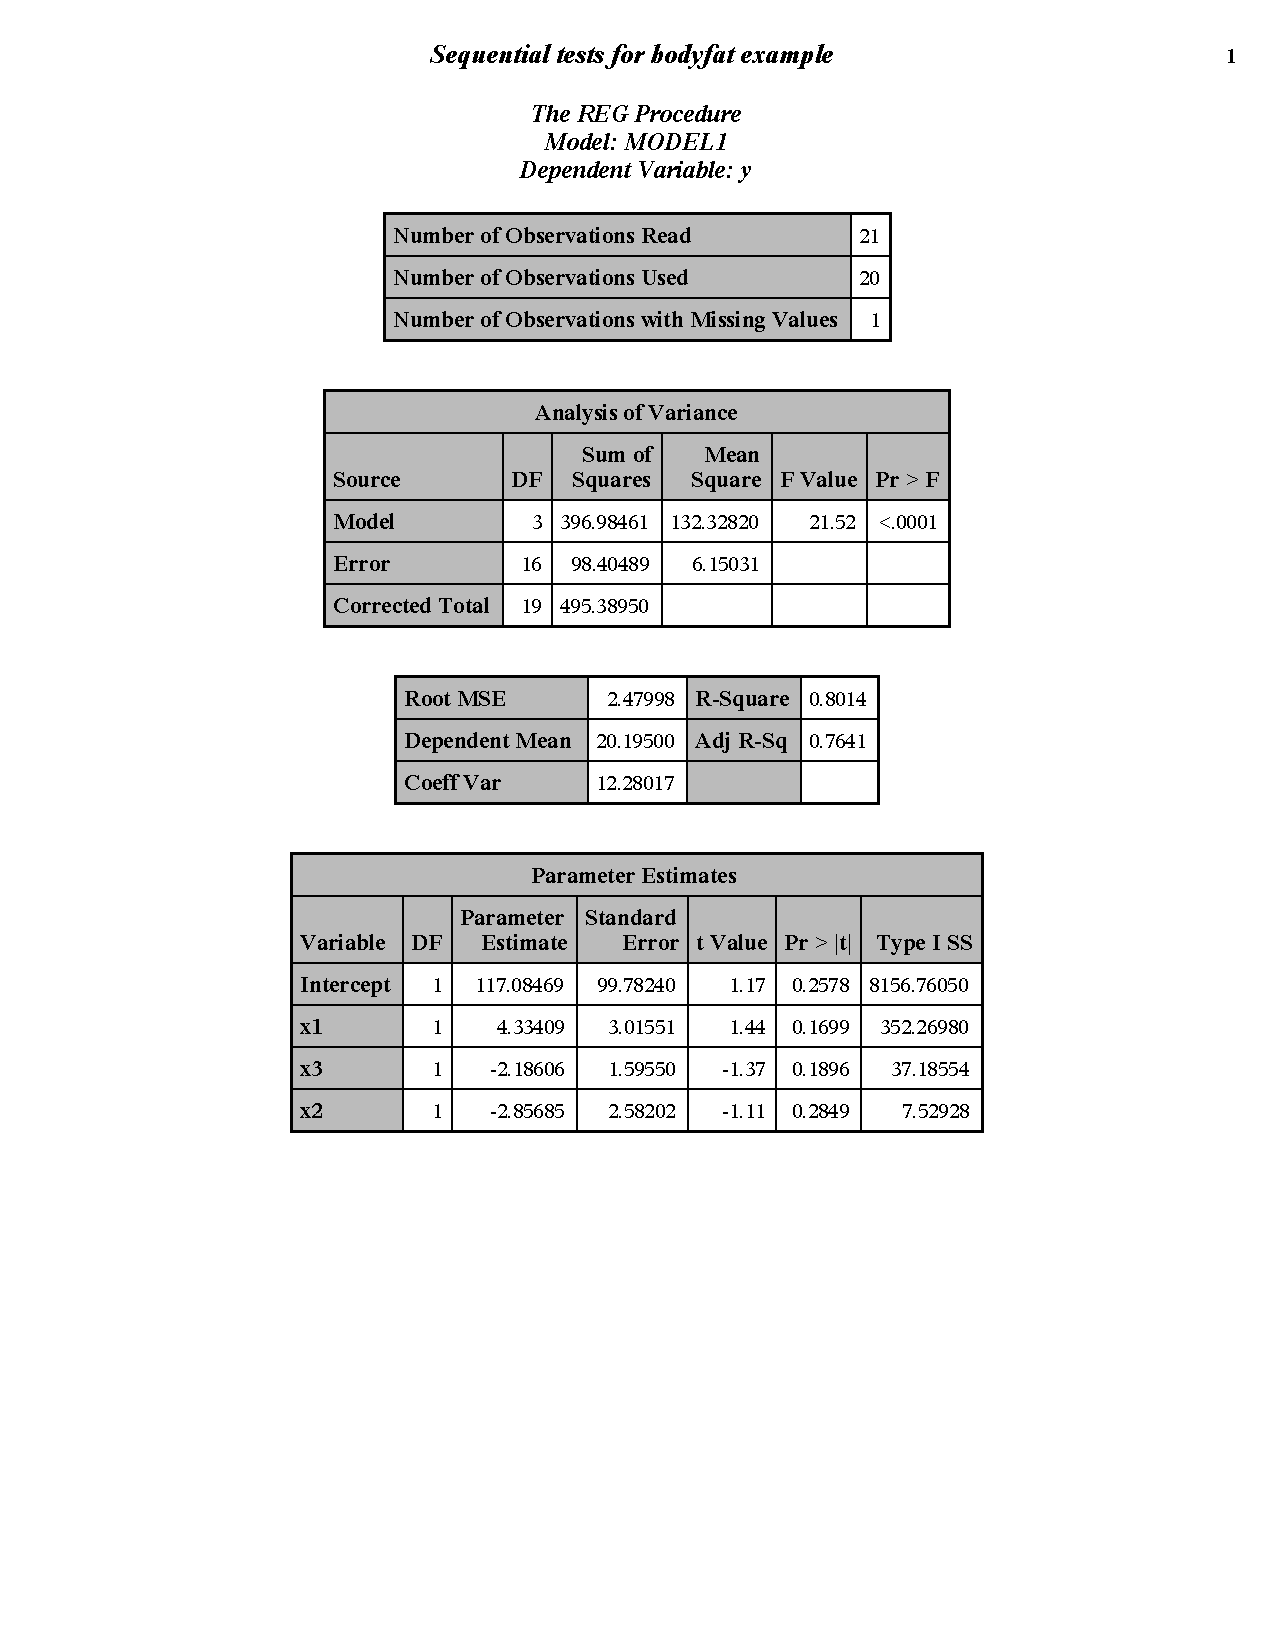
\includegraphics[page=1,scale=0.7,trim= 10mm 100mm 10mm 10mm]{bodyfatexampletypeI}
\end{center}

\newpage

Let`s label the Type I SS in terms of extra regression sums of squares (R notation).\\~\\

Note: we will soon use proc glm for our model analysis and this gives even better output for type I sums of squares.  (The tests given for type I sums of squares use the \textit{full model} MS(E) rather than the full model MS(E) up to that point.  This test still works because MS(E) from each model is an unbiased estimate of $\sigma^2$.  The tests using the different MS(E) terms could give different results, but will usually agree.\\~\\

\begin{small}
\begin{verbatim}
proc glm data=bodyfat;
   model y=x1 x3 x2;   
run;
\end{verbatim}
\end{small}

\begin{center}
\includegraphics[page=2,scale=0.7,trim= 10mm 70mm 10mm 10mm]{bodyfatexampletypeIglm}
\end{center}

\end{document}